% Tinplate Reverb - user manual (English; French: manuel.tex, same content).
% pdflatex manual.tex (three passes); figures: python3 figures.py (doc/fig_*_en.pdf).
% Copyright (C) 2026 Tinplate authors - SPDX-License-Identifier: GPL-3.0-or-later
\documentclass[a4paper,11pt]{article}
\usepackage[T1]{fontenc}
\usepackage[utf8]{inputenc}
\usepackage[english]{babel}
\usepackage{lmodern}
\usepackage{microtype}
\usepackage[margin=2.3cm]{geometry}
\usepackage{amsmath,amssymb}
\usepackage{graphicx}
\usepackage{booktabs}
\usepackage{array}
\usepackage{tabularx}
\usepackage{xcolor}
\usepackage{tikz}
\usetikzlibrary{arrows.meta,positioning,fit,calc}
\usepackage{enumitem}
\usepackage[hidelinks]{hyperref}

\definecolor{brass}{HTML}{966919}
\definecolor{steel}{HTML}{196E96}
\definecolor{ink}{HTML}{1E262D}
\definecolor{paper}{HTML}{F2F5F7}

\newcommand{\ctl}[1]{\textsf{\textbf{#1}}}   % name of an element of the interface
\newcommand{\dB}{\,dB}
\newcommand{\dBFS}{\,dBFS}
\setlist{itemsep=1pt,topsep=3pt}
\emergencystretch=3em
\graphicspath{{./}{captures/}}

\title{\textcolor{steel}{\textbf{TINPLATE}} \textsf{REVERB}\\[4pt]
\large User manual and description of the algorithm}
\author{Version 1.2.0}
\date{}

\begin{document}
\maketitle

\begin{center}
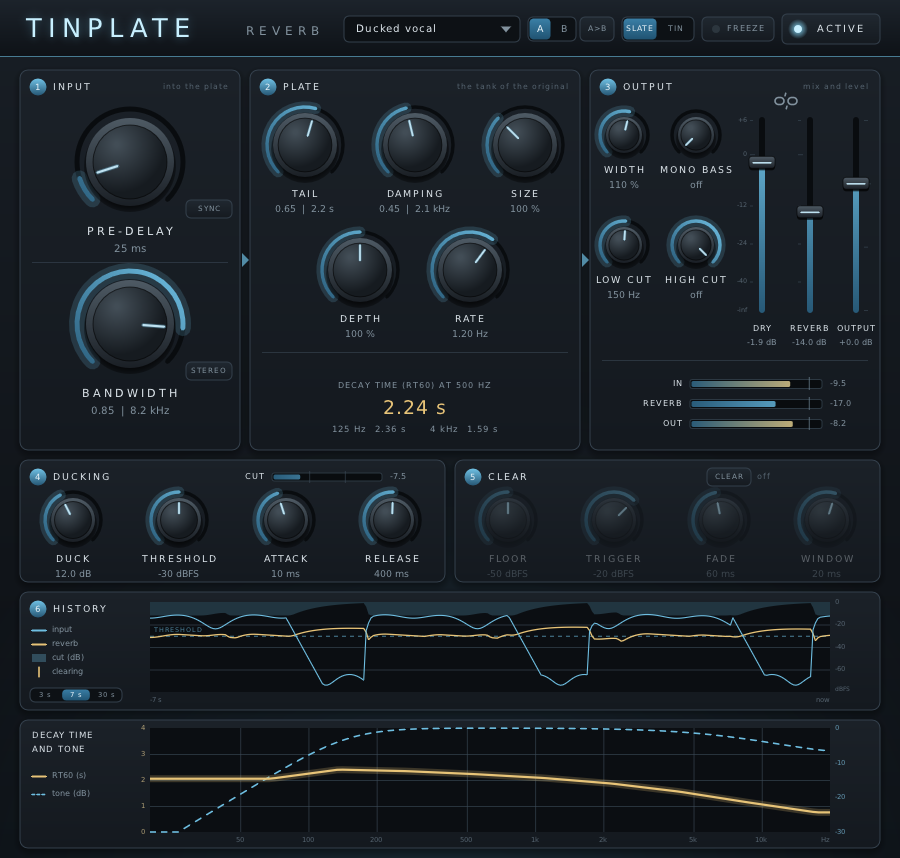
\includegraphics[width=0.92\textwidth]{capture_interface.png}
\end{center}

\newpage
\tableofcontents
\newpage

% ==============================================================================================
\section{Overview}

Tinplate Reverb is a plate reverb. Its core is that of \texttt{PlateX2} from CAPS, the LADSPA
plugin library by Tim Goetze (called \texttt{Plate2x2} in the 0.4 series), itself built on the
plate described by Jon Dattorro (\emph{Effect Design, Part 1}, J. Audio Eng. Soc., 1997). This
core is taken over unchanged, operation by operation: with the additions at neutral, the output
is that of the original to the bit (section~\ref{sec:identity}).

Around this core, Tinplate adds what everyday use needs: pre-delay (free or locked to the
tempo), size of the plate, adjustable modulation, low and high cut on the reverb, stereo width,
optional stereo input and mono bass, freeze, \emph{ducking} (the reverb steps back while the
input plays), emptying of the plate at each new attack (\emph{Clear}), tails up to 10\,s,
output gain, smoothing of the controls, display of the real decay time, history of the levels,
presets, A/B comparison.

\paragraph{Formats.} VST3 and CLAP for 64-bit Windows; VST3, CLAP and LV2 for Linux. The plugin
is stereo (two inputs, two outputs); its latency is zero.

\paragraph{Licence.} GPL 3 or later, as CAPS (file \texttt{COPYING}). The interface and the
plugin formats rely on DPF (ISC licence).

% ==============================================================================================
\section{Installation}

\paragraph{Windows.} Run \texttt{Tinplate-Reverb-1.2.0-setup.exe}: it installs the VST3
(required) and, if ticked, the CLAP and the user manuals, then adds an uninstaller (\emph{Apps
and features}). By hand: copy the folder \texttt{tinplate\_reverb.vst3} into
\verb|C:\Program Files\Common Files\VST3\| and \texttt{tinplate\_reverb.clap} into
\verb|C:\Program Files\Common Files\CLAP\|.

\paragraph{Linux.} Copy \texttt{tinplate\_reverb.vst3} into \verb|~/.vst3/|,
\texttt{tinplate\_reverb.clap} into \verb|~/.clap/| or \texttt{tinplate\_reverb.lv2} into
\verb|~/.lv2/|.

Then rescan the plugins in the host. The uninstaller leaves the preferences and the presets of
the user (section~\ref{sec:files}).

% ==============================================================================================
\section{Quick start}

\begin{enumerate}
\item \textbf{As an insert} on a track: the \ctl{Default} preset is loaded (Reverb $-16$\dB, Dry
  $-1.5$\dB, a reverb of about 1.9\,s at 500\,Hz). \textbf{On an auxiliary send}: choose
  \ctl{Send (100 \% wet)}, which gives the reverb only.
\item Set the length with \ctl{TAIL}; the value in seconds is shown under the knob and in the
  middle of section 2.
\item Darken or brighten with \ctl{DAMPING} (highs that die sooner in the tail) and
  \ctl{BANDWIDTH} (highs that enter the plate).
\item Move the reverb away from the direct sound with \ctl{PRE-DELAY} (20 to 40\,ms on a
  voice; \ctl{SYNC} locks it to the tempo); clean the low end of the mix with \ctl{LOW CUT};
  soften the highs of the tail with \ctl{HIGH CUT}.
\item Balance with the faders \ctl{DRY} (direct sound) and \ctl{REVERB} (reverb alone).
  \ctl{FREEZE} holds the reverb forever.
\item For a reverb that keeps the voice clear, raise \ctl{DUCK} (section 4): the reverb goes
  down while singing and comes back in the gaps.
\item For each new hit (chord, drum) to start in a clean reverb, switch \ctl{CLEAR} on
  (section 5). The history (section 6) shows the input and the thresholds, to set these two
  sections by eye.
\item A stereo source (piano, guitar recorded in stereo): \ctl{STEREO} (section 1); a firmer
  low end: \ctl{MONO BASS} (section 3).
\end{enumerate}

% ==============================================================================================
\section{The interface}

The window (900 × 858 points, resizable with its proportions kept, sharp on high-density
screens) reads from left to right in the order of the signal: three numbered sections joined by
arrows, then the sections \ctl{DUCKING} (4) and \ctl{CLEAR} (5), mirror images of each other,
the \ctl{HISTORY} (6) and the
plot of the decay time at the bottom. Every element has a tooltip; for a knob, its title gives
the detailed value.

\begin{center}
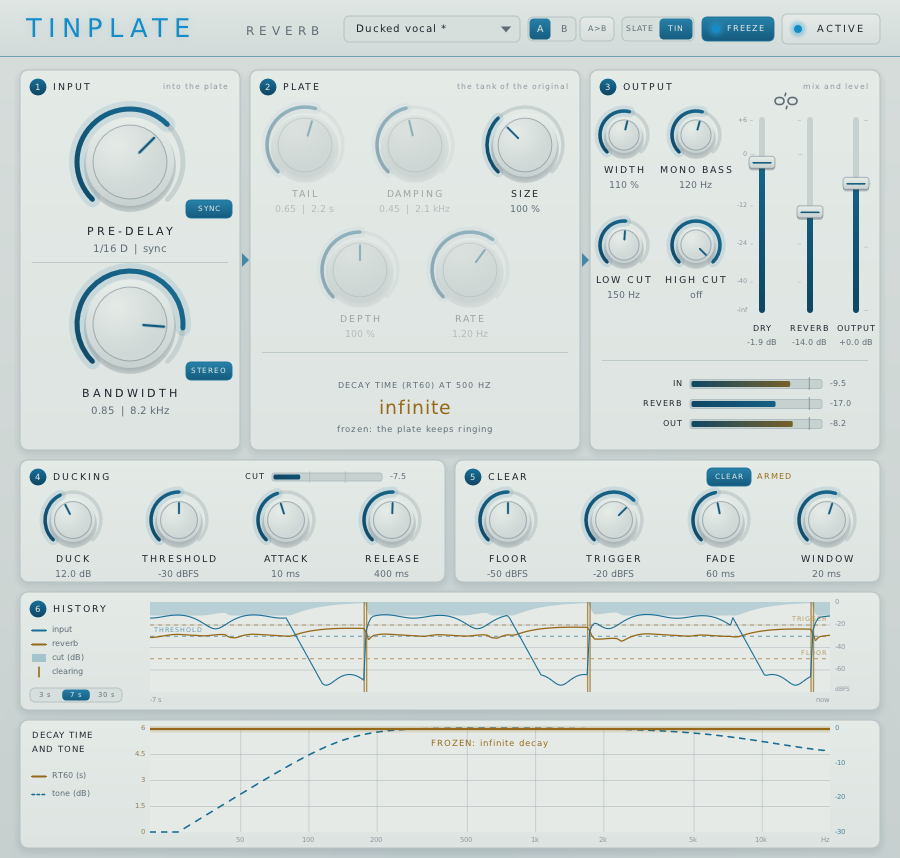
\includegraphics[width=0.8\textwidth]{capture_interface_tin.png}\\[2pt]
\small Light theme \ctl{TIN}; Freeze, Sync, stereo input, Mono bass and Clear on.
\end{center}

\subsection{Header}
\begin{description}
\item[Presets.] Drop-down list: a click opens it; it shows the factory presets
  (\ctl{FACTORY}), a line, your presets (\ctl{USER}, in alphabetical order), a line, then
  \ctl{Save current settings\ldots}. The current preset is marked with a dot; a ``*'' after
  its name means a setting was changed since it was loaded. The wheel over the closed box steps to
  the next or previous preset. Details in section~\ref{sec:presets}.
\item[A | B and A>B.] Two sets of settings to compare: a click on \ctl{A} or \ctl{B} switches
  (the set left is kept, the other one is loaded; on the first visit, B starts as a copy of A).
  \ctl{A>B} (or \ctl{B>A}) copies the current set into the other one. Both sets are saved with
  the project.
\item[SLATE | TIN.] Dark or light theme (grey with a slight green tint), no effect on the
  sound; it is a preference of the computer, shared by all instances and all projects.
\item[FREEZE.] Freezes the reverb (lit LED); Tail, Damping, Depth and Rate are then greyed,
  since they no longer act (section~\ref{sec:freeze}).
\item[ACTIVE / BYPASSED.] The Bypass declared to the host (section~\ref{sec:smoothing}).
\end{description}

\subsection{Section 1: INPUT}
\ctl{PRE-DELAY} and \ctl{BANDWIDTH}: what goes into the plate. The small \ctl{SYNC} button locks
the pre-delay to the tempo of the host: the Pre-delay knob then chooses a note value (1/64 to
1/4, dotted ``D'' or triplet ``T''). The small \ctl{STEREO} button, by Bandwidth, makes each
channel enter its own half of the plate (stereo input). Under Bandwidth, its value and the $-3$\dB{}
frequency of the filter at the current sample rate (``open'' when it stays above
$-3$\dB{} up to the Nyquist frequency).

\subsection{Section 2: PLATE}
Five knobs of the same size in two rows: \ctl{TAIL}, \ctl{DAMPING} (under it, the $-3$\dB{}
frequency of its filter) and \ctl{SIZE} (size of the plate); then \ctl{DEPTH} and \ctl{RATE}
(depth and rate of the modulation, greyed while frozen, which stops it). Below, the decay time
(RT60) at 500\,Hz, large, and at 125\,Hz and 4\,kHz (``infinite'' while frozen).

\subsection{Section 3: OUTPUT}
Four small knobs in a square: \ctl{WIDTH} and \ctl{MONO BASS} (width), \ctl{LOW CUT} and
\ctl{HIGH CUT} (tone); then three faders: \ctl{DRY} (level of the direct
sound), \ctl{REVERB} (level of the reverb alone) and \ctl{OUTPUT} (output gain). The first two
go from ``off'' (at the bottom) to $+6$\dB, with the scale on their left (0\dB{} at four
fifths of the travel); Output goes from $-24$ to $+12$\dB. The small chain above Dry and Reverb
links them (whole chain, golden) or unlinks them (broken chain): see Dry, Reverb
(section~\ref{sec:controls}). A fader follows the mouse (\textsf{Shift}: four times finer) and
otherwise works as a knob. Then three peak meters: \ctl{IN} (input), \ctl{REVERB} (reverb alone,
after Low cut, High cut, Mono bass, Width and ducking, before its fader), \ctl{OUT} (output), in dBFS;
after a peak, the display falls back with a time constant of 0.25\,s.

\subsection{Section 4: DUCKING}
\ctl{DUCK} (depth), \ctl{THRESHOLD}, \ctl{ATTACK}, \ctl{RELEASE}; the last three are greyed
while Duck is 0 (``off''), since they do not act. At the top, the \ctl{CUT} meter shows how
much the reverb is lowered now (0 to 30\dB).

\subsection{Section 5: CLEAR}
The small \ctl{CLEAR} button at the top right (off by default; the place of the \ctl{CUT} meter
in section 4) and \ctl{FLOOR}, \ctl{TRIGGER}, \ctl{FADE}, \ctl{WINDOW}, greyed while it is off.
Right of the button, the state of the detection:
``waiting'' (the input has not gone under Floor yet, or the old reverb is still fading
out), ``ARMED'' (the next attack will empty the plate), ``CLEARED'' (lit 0.2\,s at
each clearing).

\subsection{Section 6: HISTORY}
The last seconds (3, 7 or 30, chosen under the legend), in dBFS from 0 to $-80$:
\begin{itemize}
\item in steel, the peak of the \textbf{input}; in brass, that of the \textbf{reverb} after the
  ducking (before its fader);
\item shaded from the top, the \textbf{cut} of the ducking (0\dB{} at the top, in dB on the same
  scale);
\item as golden vertical lines, the \textbf{clearings} of Clear;
\item dashed, the thresholds in use: \ctl{THRESHOLD} (on the left) when Duck is not 0,
  \ctl{FLOOR} and \ctl{TRIGGER} (on the right) when Clear is on.
\end{itemize}
Threshold can thus be set on the played passages, Floor above the noise of the gaps and Trigger
under the attacks, while watching the input curve. Each point is the peak of the last
30 milliseconds, taken every 25\,ms: no peak is missed. The history is not saved with the
project.

\subsection{Decay time and tone}
At the bottom, on a frequency scale from 20\,Hz to 20\,kHz (or to the Nyquist frequency):
\begin{itemize}
\item in brass, the \textbf{decay time} against frequency (left scale, in seconds; full scale
  from 2 to 32\,s depending on the curve), set by Tail and Damping; while frozen, the words
  ``FROZEN: infinite decay'';
\item in steel and dashed, the \textbf{tone} of the reverb (right scale, in dB), set by
  Bandwidth, Low cut and High cut.
\end{itemize}

\subsection{Using the knobs}
\begin{itemize}
\item drag vertically; \textsf{Shift} for fine adjustment;
\item mouse wheel (\textsf{Shift}: fine);
\item double-click or \textsf{Ctrl}+click: default value;
\item right-click: type the value (\textsf{Enter} confirms, \textsf{Esc} cancels; a comma is
  accepted as the decimal separator); a note value (pre-delay locked to the tempo) is chosen
  with the knob or the wheel, one notch per value.
\end{itemize}

% ==============================================================================================
\section{The controls}\label{sec:controls}

\begin{center}
\small
\begin{tabularx}{\textwidth}{@{}l l l X@{}}
\toprule
Control & Range & Default & Role \\
\midrule
Pre-delay & 0--250\,ms & 0\,ms & delay before the plate \\
Sync & on/off & off & pre-delay locked to the tempo of the host \\
Note & 1/64--1/4 & 1/16 & locked pre-delay: note value (dotted, triplet) \\
Bandwidth & 0--1 & 0.5 & input low-pass of the plate (original) \\
Tail & 0--1.16 & 0.5 & length of the reverb (original up to 1) \\
Damping & 0--1 & 0.75 & low-pass inside the loop (original) \\
Size & 50--200\,\% & 100\,\% & size of the plate (100\,\%: the original) \\
Depth & 0--200\,\% & 100\,\% & depth of the modulation (100\,\%: the original) \\
Rate & 0.1--5\,Hz & 1.2\,Hz & rate of the modulation (1.2\,Hz: the original) \\
Freeze & on/off & off & reverb held forever \\
Dry & off--+6\dB & 0\dB & level of the direct sound \\
Link & on/off & off & Dry and Reverb linked as the Blend of the original \\
Mix & 0--1 & 0.25 & mix when Link is on (the Blend of the original) \\
Reverb & off--+6\dB & $-18$\dB & level of the reverb alone \\
Width & 0--200\,\% & 100\,\% & stereo width of the reverb \\
Low cut & 20\,Hz (off)--1\,kHz & off & 12\dB/octave high-pass on the reverb only \\
High cut & 1--20\,kHz (off) & off & 12\dB/octave low-pass on the reverb only \\
Stereo input & on/off & off & each channel into one half of the plate (option) \\
Mono bass & 20\,Hz (off)--500\,Hz & off & reverb mono below this frequency (option) \\
Output & $-24$--+12\dB & 0\dB & gain of the whole output \\
Duck & 0--30\dB & 0 (off) & largest cut of the reverb while the input plays \\
Threshold & $-60$--0\dBFS & $-30$\dBFS & input level where the ducking starts \\
Attack & 1--200\,ms & 10\,ms & speed of the cut \\
Release & 50--3000\,ms & 300\,ms & speed of the return \\
Clear & on/off & off & empty the plate at each new attack \\
Floor & $-80$--$-20$\dBFS & $-50$\dBFS & level under which the detection arms \\
Trigger & $-60$--0\dBFS & $-20$\dBFS & level of an attack \\
Fade & 10--500\,ms & 60\,ms & fade out of the old reverb \\
Window & 1--200\,ms & 20\,ms & longest rise of an attack \\
Bypass & on/off & off & input unprocessed, 10\,ms crossfade \\
\bottomrule
\end{tabularx}
\end{center}
The defaults of the three plate controls of the original (Bandwidth, Tail, Damping) are those a
LADSPA host gives PlateX2; the \ctl{Default} preset, loaded when the plugin opens, is different
(section~\ref{sec:presets}).

\paragraph{Pre-delay.} Delays the input of the plate: the reverb starts later than the direct
sound, which stays clearer (voice, snare). The dry sound is not delayed. A change goes from the
old delay to the new one by a 30\,ms crossfade: no pitch glide and no click.

\paragraph{Sync, Note.} With \ctl{SYNC}, the pre-delay is a note value at the tempo of the
host: from 1/64 to 1/4, with the dotted values (D, one and a half times) and the triplets (T,
two thirds), sorted by length. At 120\,BPM, 1/16 is 125\,ms and a dotted 1/8 is 375\,ms. When the
host gives no tempo, the plugin takes 120\,BPM. The delay is limited to 2\,s (a quarter note at
30\,BPM). A change of tempo or of note goes through the same 30\,ms crossfade. The Pre-delay
setting in milliseconds is kept and comes back when Sync is switched off.

\paragraph{Bandwidth.} First-order low-pass at the input of the plate: it sets how much treble
enters, hence the brightness of the whole reverb, attack included. It does not act on the
length.

\paragraph{Tail.} Gain of the loop of the plate: the larger, the longer the reverb (from 0.6
to 10\,s at 500\,Hz; figure~\ref{fig:rt60}). Even at 0, the plate rings for about 0.6\,s: its
allpass filters ring by themselves. The original stops at 1 (5.1\,s at 500\,Hz); beyond, up to
1.16, Tinplate extends the same law (loop gain $0.749 \times$ Tail, at most 0.869): 10\,s at
500\,Hz with Damping at its minimum, 6.7\,s with Damping 0.75. The lows last longer than the
highs (11.5\,s at 125\,Hz for Tail 1.16 and Damping 0.4).

\paragraph{Size.} Size of the plate: lengths of the delays of the loop and positions of the
output taps, from 50 to 200\,\% of those of the original (100\,\%: the sound of the original to
the bit). Small: more metallic, closer echoes; large: a broader plate, lower and denser
resonances. The length follows the size, as for a real plate: at the same Tail, a plate twice
as large rings about twice as long (2.1\,s at 100\,\%, 4.3\,s at 200\,\%, at 500\,Hz for Tail
0.6 and Damping 0.4; up to 18\,s at the largest Tail). A change of size glides in 100\,ms: the
pitch of the ringing reverb moves briefly, without a click. Size also acts while frozen (pitch
glide of the frozen sound).

\paragraph{Depth, Rate.} The loop of the plate is slowly modulated (a very discreet chorus),
which breaks its fixed resonances and makes the tail move. Depth sets the amount of this
modulation (0: still plate, more metallic; 200\,\%: a marked chorus, the pitch of the tail
wavers), Rate its speed (slow: floating; fast: vibrato). At the values of the original,
100\,\% and 1.2\,Hz, the sound is that of the original to the bit. A change of rate keeps the
phase of the oscillator: no click. The decay time shown is measured at Depth 100\,\%: at
Depth 0, the highs last a little longer.

\paragraph{Damping.} First-order low-pass inside the loop: at each round, the highs lose a
little more than the lows, so they die sooner (a darker, more natural sound). At 0, the loop
does not damp the highs.

\paragraph{Freeze.} The plate stops receiving the signal and losing its energy: the ringing
reverb is held forever, at the same level and with the same tone. You can play over it: the
dry signal still passes, but what is played while frozen does not enter the plate. When
released, the reverb decays again according to Tail and Damping. Details in
section~\ref{sec:freeze}.

\paragraph{Dry, Reverb.} Levels of the direct sound and of the reverb, set separately (the
original has a single Blend knob, where raising one lowers the other: wet $=
\mathrm{blend}^{1.53}$, dry $= 1 - \text{wet}$). Reverb 0\dB{} and Dry off: reverb only, for an
auxiliary send. The mix of the original at Blend 0.25 is Reverb $-18.4$\dB{} and Dry
$-1.1$\dB.

\paragraph{Dry / Reverb link.} A click on the chain between the two faders links them: this is
the Blend of the original, raising one lowers the other, the sum of their gains staying 1 (Dry
0\dB: Reverb off; Dry $-6$\dB: Reverb $-6$\dB; Dry off: Reverb 0\dB). Linked, they do not go
above 0\dB. When linking, Dry sets the mix: Reverb takes the value that completes Dry. A second
click unlinks them: the faders keep the levels they showed, without a jump. Linked, both faders
are only the display of a single control, \textbf{Mix} (0 to 1), which is exactly the Blend of
the original: reverb $\mathrm{mix}^{1.53}$, dry $1 - \mathrm{mix}^{1.53}$, to the bit. The host
sees and automates Mix; the Dry and Reverb controls are then ignored, even automated. Link and
Mix are part of the presets and of the A/B sets.

\paragraph{Width.} Stereo width of the reverb alone: 0\,\% makes it mono, 100\,\% leaves it as
it is, 200\,\% doubles the difference between the channels. The dry sound is not touched.

\paragraph{Low cut.} Second-order Butterworth high-pass (12\dB{} per octave) on the reverb
alone: it removes the lows that blur the bottom of the mix without touching the dry sound. The
knob is logarithmic; at its minimum (20\,Hz, ``off''), the filter is removed.

\paragraph{High cut.} Second-order Butterworth low-pass (12\dB{} per octave) on the reverb
alone: it darkens the tail without touching the dry sound. Unlike Bandwidth, which filters what
enters the plate, it acts on what comes out, attack included, and does not change the length;
unlike Damping, the highs do not die sooner, they are only lower. Logarithmic knob; at its
maximum (20\,kHz, ``off''), the filter is removed.

\paragraph{Stereo input.} Off (the original): the plate receives the mono sum of L and R, and
the reverb is the same wherever the source is in the panorama. On: each channel goes through its
own input filters (the same as the original's) and into one half of the plate; the start of the
reverb then follows the panning (an impulse on the left: the first 60 milliseconds on the left
only, then 2 to 4\dB{} more on the left up to 0.5\,s; figure~\ref{fig:stereo}), and the tail
comes back to the centre as with the mono input, the two halves of the plate exchanging their
energy at each round. A centred source gives exactly the same reverb either way. Switching
takes 20\,ms, without a click.

\paragraph{Mono bass.} Below the chosen frequency, the reverb is mono: the difference between
its channels goes through a second-order Butterworth high-pass (12\dB{} per octave), the sum is
not touched. The low end of the reverb is thus firmer and does not thin out in mono, without
losing the width above (at 200\,Hz: $-24$\dB{} on the difference at 50\,Hz, nothing at
2\,kHz). Width then acts on what is left of the difference. Logarithmic knob; at its minimum
(20\,Hz, ``off''), the filter is removed.

\paragraph{Output.} Gain of the whole output (dry and reverb), after the mix.

\paragraph{Duck.} The \emph{ducking} lowers the reverb while the input plays and lets it come
back in the gaps: the voice (or instrument) stays clear, and the tail is heard between the
phrases. Duck is the largest cut, in dB; at 0 (``off''), the ducking is removed and the
output is exactly that without ducking. The frozen reverb (Freeze) is lowered the same way. The
dry sound is never touched.

\paragraph{Threshold.} Peak level of the input (dBFS) where the ducking starts: the reverb is
cut by as many dB as the input goes over this threshold, at most by Duck. With Threshold
$-30$\dBFS{} and Duck 12\dB, an input at $-24$\dBFS{} cuts the reverb by 6\dB, an input at
$-18$\dBFS{} or more by 12\dB.

\paragraph{Attack, Release.} Speeds of the cut and of the return (time constants). Short
Release: the reverb comes back up in every small gap (between two words); long: it waits for the
end of the phrase (figure~\ref{fig:duck}).

\paragraph{Clear.} When a new sound comes after a silence, the old reverb fades out in Fade
milliseconds and the new sound starts in an empty plate: each chord, each hit has its own
reverb, without the tail of the previous one. An attack is a rise of the input from under Floor
to over Trigger in less than Window milliseconds; a slower rise (crescendo, fade in) does not
empty the plate. After a clearing, the detection arms again only once the fade has ended and
the input has gone back under Floor. While frozen (Freeze), nothing is emptied: the frozen sound
is kept. Off, Clear changes nothing to the sound.

\paragraph{Floor, Trigger, Fade, Window.} Floor must be above the noise of the gaps between the
notes (the reverb does not enter the detection: only the input signal counts), Trigger under the
level of the attacks. Short Window (5 to 20\,ms): only sharp attacks (drums, plucked strings)
empty the plate; long (50 to 200\,ms): softer attacks too. Short Fade: a clean cut of the old
tail; long: a softer transition.

% ==============================================================================================
\section{Presets}\label{sec:presets}

\subsection{Factory presets}
\begin{center}
\small
\begin{tabular}{@{}l r r r r r r r r r r@{}}
\toprule
Name & Bandw. & Tail & Damp. & Reverb & Dry & Pre-d. & Low cut & Width & Duck & RT60 \\
\midrule
Default           & 0.80 & 0.55 & 0.40 & $-16.0$ & $-1.5$ & 12 & 60  & 100 & off & 1.9 \\
Original (CAPS)   & 0.50 & 0.50 & 0.75 & $-18.4$ & $-1.1$ & 0  & off & 100 & off & 1.6 \\
Vocal plate       & 0.85 & 0.45 & 0.45 & $-18.4$ & $-1.1$ & 35 & 150 & 110 & off & 1.7 \\
Drum plate        & 0.90 & 0.30 & 0.30 & $-20.1$ & $-0.9$ & 5  & 200 & 120 & off & 1.3 \\
Ambience          & 0.70 & 0.15 & 0.50 & $-21.4$ & $-0.8$ & 0  & 100 & 130 & off & 0.9 \\
Dark and long     & 0.55 & 0.85 & 0.75 & $-14.0$ & $-1.9$ & 20 & 60  & 100 & off & 2.9 \\
Bright and wide   & 1.00 & 0.70 & 0.10 & $-16.0$ & $-1.5$ & 15 & 120 & 150 & off & 2.6 \\
Send (100 \% wet) & 0.80 & 0.60 & 0.40 & 0 & off & 20 & 100 & 100 & off & 2.1 \\
Ducked vocal      & 0.85 & 0.65 & 0.45 & $-14.0$ & $-1.9$ & 25 & 150 & 110 & 12  & 2.2 \\
Piano (clear)     & 0.80 & 0.70 & 0.45 & \multicolumn{2}{c}{Mix 0.30} & 15 & 80 & 120 & off & 2.9 \\
Snare (clear)     & 0.95 & 0.50 & 0.25 & \multicolumn{2}{c}{Mix 0.25} & 1/32 & 200 & 130 & off & 1.6 \\
Guitar (stereo)   & 0.80 & 0.60 & 0.40 & \multicolumn{2}{c}{Mix 0.28} & 20 & 120 & 140 & off & 2.3 \\
\bottomrule
\end{tabular}
\end{center}
Reverb and Dry in dB (the mix of the original at Blend 0.30, 0.25, 0.22\ldots), Pre-delay in
ms, Low cut in Hz, Width in \%, Duck in dB, RT60 at 500\,Hz in seconds (at 44.1\,kHz); Output at
0\dB{} everywhere, Freeze off, High cut off; Threshold $-30$\dBFS{} and Attack 10\,ms
everywhere, Release 300\,ms (400\,ms for Ducked vocal); Size 100\,\%, Clear, Link, Sync and the
options off, except for the last three. \textbf{Piano (clear)}: Size 120\,\%, Link (Mix 0.30),
Clear (Floor $-50$, Trigger $-20$\dBFS, Fade 120\,ms, Window 40\,ms), stereo input.
\textbf{Snare (clear)}: Size 90\,\%, Link (Mix 0.25), High cut 12\,kHz, pre-delay locked to a
thirty-second note (1/32), Clear (Floor $-45$, Trigger $-15$\dBFS, Fade 40\,ms, Window 10\,ms).
\textbf{Guitar (stereo)}: Size 110\,\%, Depth 120\,\%, Rate 0.8\,Hz, Link (Mix 0.28), stereo
input, Mono bass 150\,Hz. ``Original (CAPS)'' reproduces the original to the bit. These
presets were set from the laws of the controls, not by ear. They are also given to the host
(list of programs).

\subsection{Your presets}
\begin{description}
\item[Save.] In the list, \ctl{Save current settings\ldots}, then type the name directly in
  the box (proposed: the name of your current preset). \textsf{Enter} saves, \textsf{Esc} or a
  click elsewhere cancels. A hint says what \textsf{Enter} will do: save, replace your preset of
  the same name (upper and lower case alike), or refuse: name of a factory preset, invalid name,
  folder not writable. Names: 1 to 24 printable ASCII characters, without
  \verb|< > : " / \ | ? *|, no space or dot at the start or at the end, no reserved Windows name
  (\texttt{CON}, \texttt{NUL}\ldots).
\item[Delete.] Hover over your preset in the list: a cross appears on the right. A first click
  shows ``delete?'', a second one deletes (no undo).
\item[Scope.] Your presets are shared by all projects, all instances and all hosts of the
  computer; the list is read again each time it opens, the file each time it is loaded. The host
  only sees the factory presets; its own presets (for example \texttt{.vstpreset}) remain
  possible and independent.
\end{description}
Freeze and Bypass, which are for playing and listening, are part of no preset and of no A/B
set.

% ==============================================================================================
\section{The algorithm}

This section describes exactly what the plugin computes (files
\nolinkurl{plugin/TinplatePlugin.cpp} and \nolinkurl{plugin/PlateCore.hpp}). The figures are
computed with the same formulas and, for the impulse responses, with the code of the plate
itself.

\subsection{Signal flow}

\begin{center}
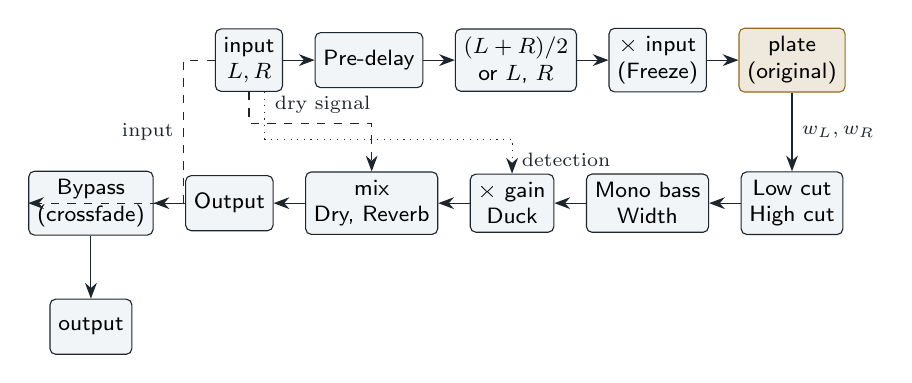
\begin{tikzpicture}[
  node distance=4mm and 4mm,
  blk/.style={draw=ink, rounded corners=2pt, fill=paper, minimum height=7mm, align=center,
              font=\footnotesize\sffamily, inner sep=3pt},
  core/.style={blk, fill=brass!15, draw=brass},
  arr/.style={-{Stealth[length=2mm]}, ink}]
\node[blk] (in) {input\\$L, R$};
\node[blk, right=of in] (pre) {Pre-delay};
\node[blk, right=of pre] (sum) {$(L+R)/2$\\or $L$, $R$};
\node[blk, right=of sum] (frz) {× input\\(Freeze)};
\node[core, right=of frz] (plate) {plate\\(original)};
\node[blk, below=10mm of plate] (lc) {Low cut\\High cut};
\node[blk, left=of lc] (wd) {Mono bass\\Width};
\node[blk, left=of wd] (dk) {× gain\\Duck};
\node[blk, left=of dk] (mix) {mix\\Dry, Reverb};
\node[blk, left=of mix] (out) {Output};
\node[blk, left=of out] (byp) {Bypass\\(crossfade)};
\node[blk, below=8mm of byp] (s) {output};
\draw[arr] (in) -- (pre); \draw[arr] (pre) -- (sum); \draw[arr] (sum) -- (frz);
\draw[arr] (frz) -- (plate); \draw[arr] (plate) -- node[right, font=\scriptsize] {$w_L, w_R$} (lc);
\draw[arr] (lc) -- (wd); \draw[arr] (wd) -- (dk); \draw[arr] (dk) -- (mix);
\draw[arr] (mix) -- (out); \draw[arr] (out) -- (byp); \draw[arr] (byp) -- (s);
\draw[arr, dashed] (in.south) -- ++(0,-4mm) -| node[pos=0.3, above, font=\scriptsize] {dry signal} (mix.north);
\draw[arr, dotted] (in.south) ++(2mm,0) -- ++(0,-6mm) -| node[pos=0.8, right, font=\scriptsize] {detection} (dk.north);
\draw[arr, dashed] (in.west) -- ++(-4mm,0) |- node[pos=0.25, left, font=\scriptsize] {input} (byp.west);
\end{tikzpicture}
\end{center}

The Pre-delay delays both channels. The input is then brought to mono, as in the original, with
a constant of $\pm10^{-20}$ ($-400$\dB, its sign flipped at each sample) that keeps the plate out
of denormal numbers; with the stereo input, $L$ and $R$ enter separately
(section~\ref{sec:stereo}). The plate gives two channels, $w_L$ and $w_R$. All the rest is
stereo.

\subsection{The plate}\label{sec:plate}

\begin{center}
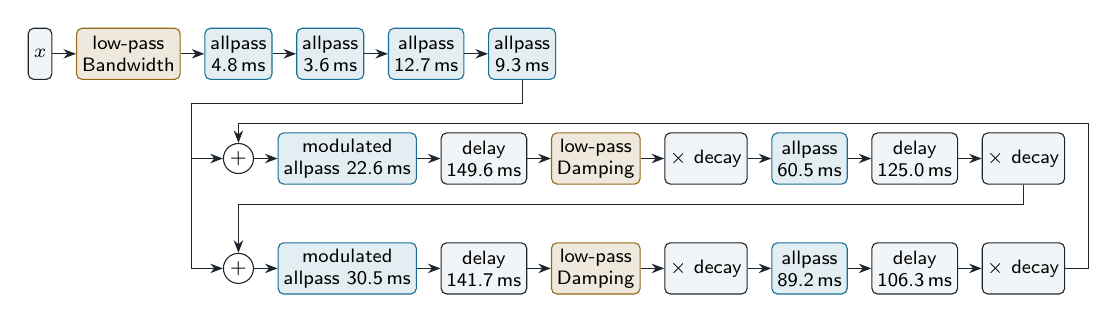
\begin{tikzpicture}[
  node distance=3mm and 3mm,
  blk/.style={draw=ink, rounded corners=2pt, fill=paper, minimum height=6.5mm, align=center,
              font=\scriptsize\sffamily, inner sep=2pt},
  ap/.style={blk, fill=steel!12, draw=steel},
  lp/.style={blk, fill=brass!15, draw=brass},
  arr/.style={-{Stealth[length=1.6mm]}, ink}]
\node[blk] (x) {$x$};
\node[lp, right=of x] (bw) {low-pass\\Bandwidth};
\node[ap, right=of bw] (d1) {allpass\\4.8\,ms};
\node[ap, right=of d1] (d2) {allpass\\3.6\,ms};
\node[ap, right=of d2] (d3) {allpass\\12.7\,ms};
\node[ap, right=of d3] (d4) {allpass\\9.3\,ms};
\node[circle, draw=ink, inner sep=1pt, font=\scriptsize, below=8mm of d1] (sL) {$+$};
\node[ap, right=of sL] (mL) {modulated\\allpass 22.6\,ms};
\node[blk, right=of mL] (tL) {delay\\149.6\,ms};
\node[lp, right=of tL] (dL) {low-pass\\Damping};
\node[blk, right=of dL] (gL) {× decay};
\node[ap, right=of gL] (aL) {allpass\\60.5\,ms};
\node[blk, right=of aL] (uL) {delay\\125.0\,ms};
\node[blk, right=of uL] (hL) {× decay};
\node[circle, draw=ink, inner sep=1pt, font=\scriptsize, below=10mm of sL] (sR) {$+$};
\node[ap, right=of sR] (mR) {modulated\\allpass 30.5\,ms};
\node[blk, right=of mR] (tR) {delay\\141.7\,ms};
\node[lp, right=of tR] (dR) {low-pass\\Damping};
\node[blk, right=of dR] (gR) {× decay};
\node[ap, right=of gR] (aR) {allpass\\89.2\,ms};
\node[blk, right=of aR] (uR) {delay\\106.3\,ms};
\node[blk, right=of uR] (hR) {× decay};
\draw[arr] (x) -- (bw); \draw[arr] (bw) -- (d1); \draw[arr] (d1) -- (d2); \draw[arr] (d2) -- (d3);
\draw[arr] (d3) -- (d4);
\draw[arr] (d4.south) -- ++(0,-3mm) -| ($(sL.west)+(-4mm,0)$) -- (sL.west);
\draw[arr] ($(sL.west)+(-4mm,0)$) |- (sR.west);
\draw[arr] (sL) -- (mL); \draw[arr] (mL) -- (tL); \draw[arr] (tL) -- (dL); \draw[arr] (dL) -- (gL);
\draw[arr] (gL) -- (aL); \draw[arr] (aL) -- (uL); \draw[arr] (uL) -- (hL);
\draw[arr] (sR) -- (mR); \draw[arr] (mR) -- (tR); \draw[arr] (tR) -- (dR); \draw[arr] (dR) -- (gR);
\draw[arr] (gR) -- (aR); \draw[arr] (aR) -- (uR); \draw[arr] (uR) -- (hR);
\draw[arr] (hL.south) -- ++(0,-2.5mm) -| (sR.north);
\draw[arr] (hR.east) -- ++(3mm,0) |- ($(sL.north)+(0,2.5mm)$) -- (sL.north);
\end{tikzpicture}
\end{center}

\paragraph{Input diffusion.} After the Bandwidth low-pass, four allpass filters in series
(coefficients 0.742, 0.742, 0.712, 0.712) spread the impulse into a cloud of dense echoes before
the loop.

\paragraph{Tank.} Two cross-coupled halves: the output of each half, times $\mathrm{decay}$, is
added to the input of the other one. Each half chains an allpass whose delay is modulated
(coefficient 0.723), a delay, the Damping low-pass, the decay gain, an allpass (0.729), a delay
and the decay gain again. A full round of both halves lasts 725\,ms; it goes four times through
the decay gain and twice through Damping. The delays (in milliseconds above) are those of the
original and follow the sample rate.

\paragraph{Modulation.} The two modulated allpasses read their delay with linear interpolation,
moved by a 1.2\,Hz sine of amplitude 0.4\,ms ($\pm 17$ samples at 44.1\,kHz), in quadrature from
one half to the other; Rate sets the frequency, Depth multiplies the amplitude (0 to 2, memory
reserved for 2). When Rate changes, the recursive oscillator ($y_n = 2\cos\omega\, y_{n-1} -
y_{n-2}$) is set again at the new frequency with the phase it had, taken from its last two
values; Depth changes in 200\,ms. This slow variation breaks the fixed resonances of the loop
(a metallic sound, says Dattorro) and gives the tail its motion.

\paragraph{Outputs.} Each channel is the sum of six taps in the delays and allpasses of both
halves, with alternating signs, times 0.6. The taps of the two channels being different, the
reverb is stereo even for a mono input (figure~\ref{fig:response}).

\paragraph{Stereo input.}\label{sec:stereo} The plate has a second set of input filters (the
Bandwidth low-pass and four allpasses, the same). With $t$ going from 0 to 1 in 20\,ms when the
option is switched on (from 1 to 0 when it is switched off), the right half of the tank receives
$d_a$ and the left half $d_a + t\,(d_b - d_a)$, where $d_a$ is the diffusion of $x + t\,(L - x)$
($x = (L+R)/2$) and $d_b$ that of $R$. At $t = 0$ this is the original; at $t = 1$, $L$ feeds
the right half, whose taps make most of the left output, and $R$ the left half. The filters
being linear and identical, an input $L = R$ gives the same output as in mono (checked to the
bit). With the option off, the second set does not compute and is emptied.

\begin{figure}[htbp]
\centering
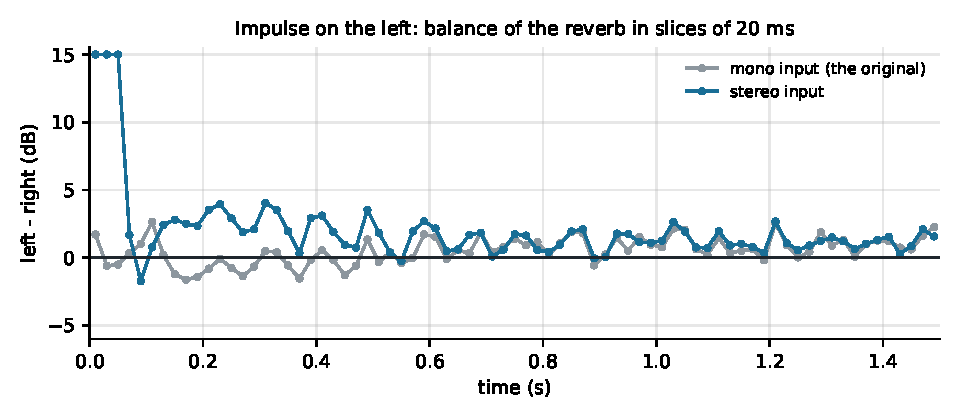
\includegraphics[width=0.8\textwidth]{fig_stereo_en.pdf}
\caption{Impulse on the left channel only: level difference between the channels of the reverb,
in slices of 20\,ms (Bandwidth 0.8, Tail 0.55, Damping 0.4; the first value is limited to
15\dB). The mono input already leans a little to the left: the taps of the two channels are
not symmetric.}
\label{fig:stereo}
\end{figure}

\paragraph{Size.} The lengths of the four delays, of the two allpasses and of the two modulated
allpasses of the loop, and the positions of the twelve output taps, are those of the original
times Size, rounded to the sample; the four input diffusers do not change (the attack keeps its
texture). The memory is reserved for 200\,\%. A delay reads the sample written $n$ steps
before, as the read pointer of the original: at 100\,\%, the values read are exactly those of
the original. The loop gain is not compensated: a longer round loses as much per round, so the
length grows about as the size. When Size changes, each length goes linearly to its new integer
value in 100\,ms; during this glide only, the reads are linearly interpolated (hence the brief
pitch glide). With Clear, the empty plate that takes over goes at once to the current size.

\paragraph{Laws of the controls.} These are those of the original (figure~\ref{fig:laws}), with
$p$ the value of the knob (Tail up to 1.16):
\[
a_{\mathrm{bw}} = e^{-\pi\,(1 - (0.005 + 0.994\,p))}, \qquad
\mathrm{decay} = 0.749\,p, \qquad
a_{\mathrm{damp}} = e^{-\pi\,(0.0005 + 0.9995\,p)},
\]
where $a$ is the coefficient of the low-pass $y[n] = a\,x[n] + (1-a)\,y[n-1]$. Its $-3$\dB{}
frequency, shown by the interface, depends on the sample rate $f_s$:
\[
\cos\frac{2\pi f_{-3}}{f_s} = \frac{1 + (1-a)^2 - 2a^2}{2\,(1-a)} .
\]

\begin{figure}[htbp]
\centering
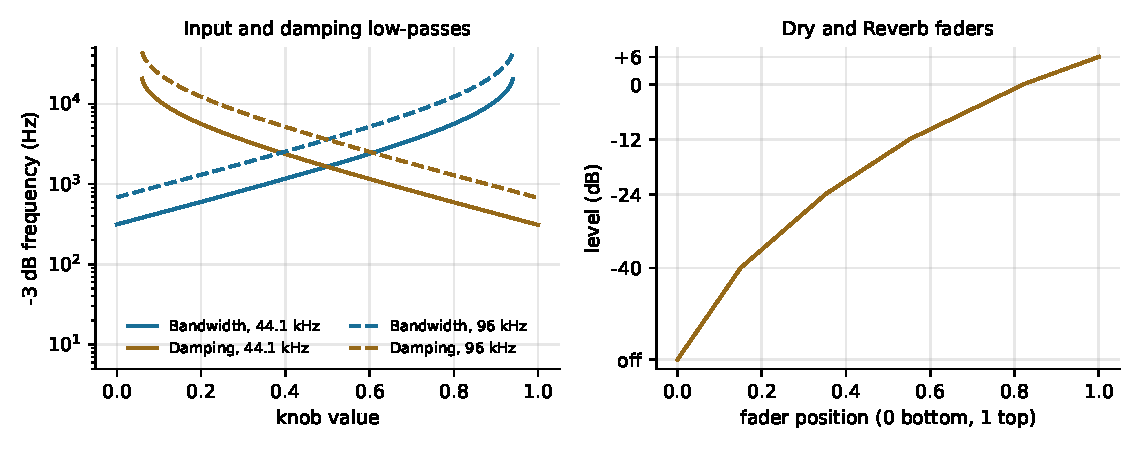
\includegraphics[width=\textwidth]{fig_lois_en.pdf}
\caption{Left: $-3$\dB{} frequency of the Bandwidth and Damping low-passes (a curve stops when
the filter stays above $-3$\dB{} up to the Nyquist frequency). Right: level in dB of the Dry
and Reverb faders against their position.}
\label{fig:laws}
\end{figure}

\paragraph{Sample rate.} The coefficients of the filters do not depend on $f_s$, the delays do.
At 96\,kHz, Bandwidth and Damping thus cut twice as high as at 48\,kHz, as in the original, and
the decay time at a frequency $f$ is the one at $f \times 44\,100/f_s$ at 44.1\,kHz. The
interface shows the real values at the current rate.

\begin{figure}[htbp]
\centering
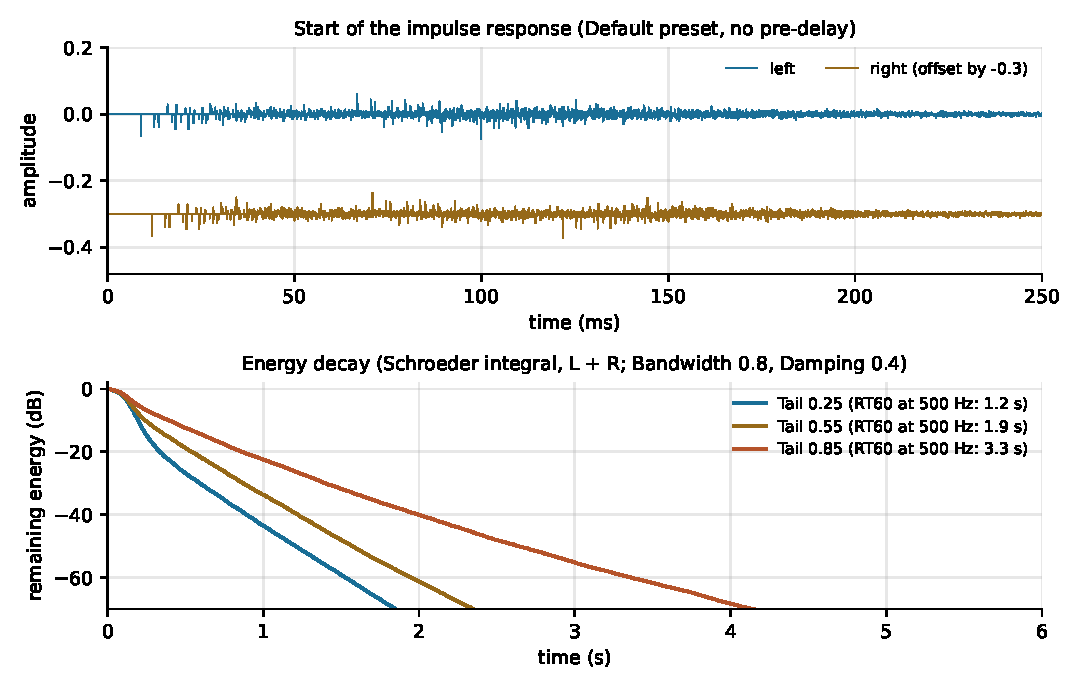
\includegraphics[width=\textwidth]{fig_reponse_en.pdf}
\caption{Top: the first 250 milliseconds of the impulse response of the plate, two channels.
Bottom: remaining energy, wide band; the fast fall of the first tenths of a second comes from
the highs, which die sooner through Bandwidth and Damping.}
\label{fig:response}
\end{figure}

\subsection{Decay time}\label{sec:rt60}

The decay time (RT60) is the time the reverb takes to lose 60\dB. Computing it from the loop
gain alone (decay$^4$ and two passes through Damping per round of 725\,ms) gives 20 to 60\,\%
less than reality: the allpasses of the tank, with coefficients near 0.72, ring by themselves
(0.5 to 0.65\,s even at Tail 0) and their group delay varies with frequency.

The interface therefore shows \textbf{measured} values: a table of the impulse response of the
plate at 44.1\,kHz, for 4 sizes (50, 100, 150 and 200\,\%), 25 values of Tail (0 to 1.2 in steps
of 0.05), 9 of Damping and 9 octave bands from 62.5\,Hz to 16\,kHz. For each point, the response
(sum of both channels) goes through a band-pass ($Q = 2$); its energy is integrated from the end
(Schroeder integral) and the slope between $-5$ and $-25$\dB{} is extended to 60\dB. Between the
points, the table is linearly interpolated; a measurement made again between the points of the
grid differs from the value shown by less than 10\,\% (at most 7.6\,\% on the 15 cases checked,
three of them with Tail beyond 1: 9.87\,s measured for 9.94\,s shown at Tail 1.16, and five at
other sizes, between the sizes measured: 75, 130, 175\,\%\ldots).

\begin{figure}[htbp]
\centering
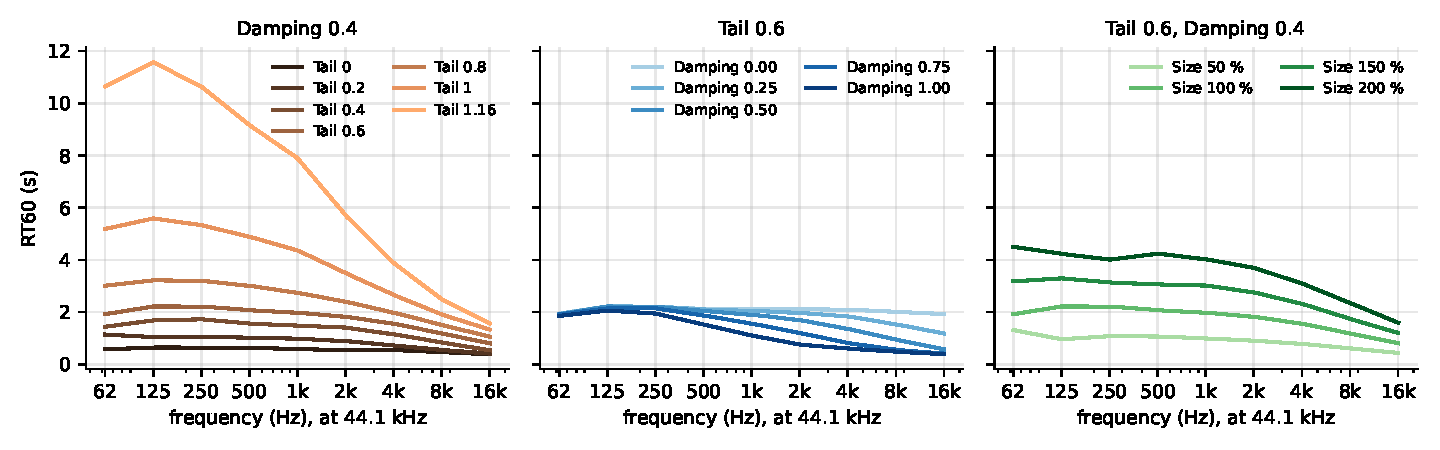
\includegraphics[width=\textwidth]{fig_rt60_en.pdf}
\caption{Decay time against frequency (measured table, at 44.1\,kHz): left against Tail,
middle against Damping, right against Size.}
\label{fig:rt60}
\end{figure}

Figure~\ref{fig:rt60} shows the two roles: Tail lengthens the reverb at all frequencies;
Damping mostly shortens the highs and leaves the lows nearly unchanged.

\subsection{Tone: Bandwidth, Low cut and High cut}

\paragraph{Low cut.} Second-order Butterworth high-pass (Robert Bristow-Johnson's form,
$Q = 1/\sqrt 2$), computed in double precision, on both channels of the reverb; its frequency
is limited to $0.45\,f_s$. At its minimum, its coefficients are those of the identity and it is
bypassed as soon as its state has emptied: the output is then exactly the unfiltered reverb. The
tone curve of the interface (figure~\ref{fig:tone}) is the product of the response of Bandwidth
and of those of analogue Butterworth filters at the same frequencies.

\paragraph{High cut.} Second-order Butterworth low-pass, of the same form, after the Low cut;
its frequency is limited to $0.45\,f_s$. At its maximum, it is bypassed the same way.

\begin{figure}[htbp]
\centering
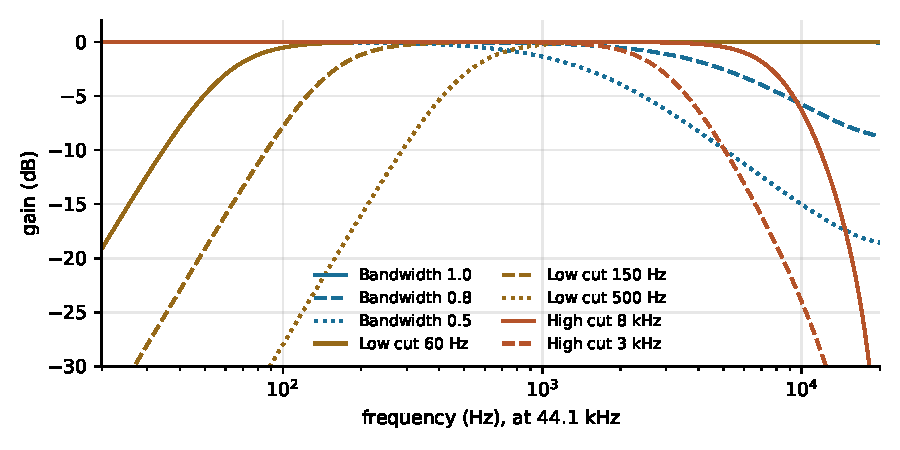
\includegraphics[width=0.75\textwidth]{fig_ton_en.pdf}
\caption{Response of the input low-pass (Bandwidth), of the low cut and of the high cut of the
reverb, at 44.1\,kHz.}
\label{fig:tone}
\end{figure}

\subsection{Mono bass, width, mix and output}

With $m = (w_L + w_R)/2$, $s = (w_L - w_R)/2$, $H$ the Mono bass high-pass (second-order
Butterworth, same form as the Low cut, applied to $s$ alone; the identity when ``off'') and
$W$ the width (Width/100):
\[
w'_L = m + W\,H(s), \qquad w'_R = m - W\,H(s) .
\]
Then, with $g_w = 10^{\mathrm{Reverb}/20}$, $g_d = 10^{\mathrm{Dry}/20}$ (0 at ``off'',
exactly 1 at 0\dB) and $G = 10^{\mathrm{Output}/20}$:
\[
y_{L,R} = \bigl(g_w\, w'_{L,R} + g_d\, x_{L,R}\bigr)\, G ,
\]
where $x_{L,R}$ is the input, not delayed: the latency is zero. With the ducking, $w'_{L,R}$ is
multiplied before the mix by the gain $10^{-c/20}$ described below.

\subsection{Ducking}\label{sec:duck}

At each sample, the detector takes the peak of the input, $e = \max(|x_L|, |x_R|)$, before the
Pre-delay, and derives the target cut, in dB:
\[
c^\ast = \min\bigl(\max(20 \log_{10} e - T,\; 0),\; D\bigr),
\]
with $T$ the threshold (Threshold) and $D$ the depth (Duck). The cut $c$ follows $c^\ast$
through a first-order filter in dB, with the time constant Attack when it grows and Release
when it shrinks:
\[
c_n = c^\ast_n + a\,(c_{n-1} - c^\ast_n), \qquad a = e^{-1/(\tau f_s)},\quad
\tau = \begin{cases} \text{Attack} & c^\ast_n > c_{n-1} \\ \text{Release} & \text{otherwise.}\end{cases}
\]
The reverb is multiplied by $10^{-c/20}$. When $c^\ast$ is zero and $c$ has fallen under
$10^{-3}$\dB{} (a gain of $1 - 1.2\times10^{-4}$), $c$ is set to zero and the gain is no longer
applied: the output is again exactly that without ducking (checked: identical to the bit 2.8\,s
after the end of the input for a cut of 12\dB{} and Release 300\,ms). The controls act at once,
without a ramp: the filter already smooths the cut. The plate itself is not touched: only its
output is lowered, so the tail comes back at the level it would have had without ducking.

\subsection{Clearing (Clear)}\label{sec:clear}

The plugin has two identical plates. The input goes into the current plate. At an attack, the
other plate, empty, becomes the current one and receives the input from that very sample; the
old one receives nothing more and its output fades out in Fade milliseconds (raised cosine,
$g = \tfrac12 + \tfrac12 \cos(\pi t / \text{Fade})$), then it is emptied and stops computing.
Both plates compute together only during the fade. After the fade, the output is exactly that of
a fresh plate that would have received the new sound only (checked to the bit).

Detection: peak envelope $e_n = \max(\max(|x_L|,|x_R|),\; e_{n-1} e^{-1/(0.03 f_s)})$ of the
input before the Pre-delay (instant rise, fall with a time constant of 30\,ms, which covers the
zero crossings of a held note). The detection arms when $e$ is under Floor and no fade is
running; armed, it triggers if $e$ goes over Trigger less than Window milliseconds after going
over Floor, and disarms otherwise. The samples between the crossing of Floor and that of Trigger
(at most Window, usually a few samples for a sharp attack) still go into the old plate. Off,
Clear runs the first plate only: the output is identical to the bit to that without Clear.

\begin{figure}[htbp]
\centering
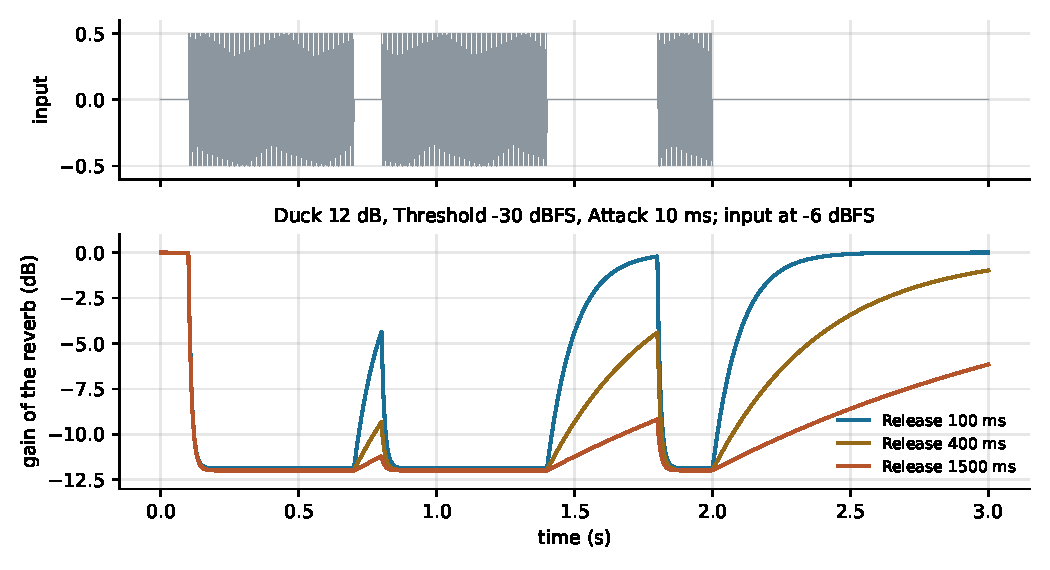
\includegraphics[width=0.85\textwidth]{fig_duck_en.pdf}
\caption{Gain of the reverb during three phrases separated by gaps of 0.1, 0.4 and 1\,s, for
three values of Release (computation of the plugin made again in NumPy).}
\label{fig:duck}
\end{figure}

\subsection{History}
The plugin gives the interface, at each block, the peak of the input, that of the reverb after
the ducking and the largest cut of the ducking over the last 30 milliseconds (eight bins of
5\,ms, the last seven of which are read, whatever the block size), and the count of the
clearings of Clear. The interface takes these values every 25\,ms and keeps 30\,s (1201
points); a clearing is marked when the count has changed since the previous point. None of this
touches the sound.

\subsection{Freeze}\label{sec:freeze}

When Freeze is switched on, in 20\,ms: the input of the plate closes, the decay gain goes to 1
and the Damping low-pass is removed; in 200\,ms: the depth of the modulation goes to 0. The loop
is then made of allpasses and integer delays only, which keep the energy at every frequency:
the level stays constant within $\pm0.3$\dB{} over 20\,s from 100\,Hz to 16\,kHz.

Without stopping the modulation, the linear interpolation of the modulated delays would lose the
highs while frozen ($-11$\dB{} at 8\,kHz and $-16$\dB{} at 16\,kHz in 10\,s).

When released, the same ramps bring Tail, Damping, the input and the modulation back to their
values: the frozen reverb then decays normally.

\subsection{Smoothing of the controls and Bypass}\label{sec:smoothing}

The original applies a change of a control at the next audio block, at once: turning Tail or
Blend while playing gives zipper noise (a jump of 0.76 on a sine of amplitude 0.5 when Blend
goes from 0 to 1). Here, each coefficient (Bandwidth, decay, Damping, gains of Dry and Reverb,
width, Output, coefficients of the Low cut and of the High cut) goes linearly to its new value in
20\,ms, then takes it exactly (same case, Dry off and Reverb 0\dB{} at once: a jump of 0.025).
The Pre-delay changes by a 30\,ms crossfade; a new change waits for the end of the crossfade.
The stereo input switches by a 20\,ms ramp (section~\ref{sec:stereo}).

\paragraph{Bypass.} The output becomes the input, exactly, through a 10\,ms crossfade. The plate
keeps running during the Bypass.

\subsection{Identity with the original}\label{sec:identity}

The code of the plate is a transcription of that of CAPS 0.9.26 (classes \texttt{PlateStub},
\texttt{Delay}, \texttt{LP1}, \texttt{Sine}) that keeps the type of each operation (samples in
single precision, some products and sums in double). With Pre-delay 0, Low cut and High cut
off, Width 100\,\%, Output 0\dB, Size and Depth 100\,\%, Rate 1.2\,Hz, Duck 0, Clear, Freeze,
Stereo input and Mono bass off, for any values of Bandwidth, Damping and Tail (up to 1), the
output is \textbf{that of the original to the bit} with Link on and Mix equal to the Blend of
the original, for any mix, with steady controls; likewise, without Link, for the reverb alone
(Reverb 0\dB, Dry off) and for the direct sound alone (Dry 0\dB, Reverb off). Without Link, for
a mix, the gains of the faders, computed from dB, do not fall exactly on
$\mathrm{blend}^{1.53}$: the gap is that of rounding ($1.3\times10^{-7}$ of the peak at most over
20 mixes). This is checked at every build against the source code of CAPS itself, called as a
LADSPA host would: 60 cases to the bit and 20 mixes (7 settings at 44.1, 48, 96 and 192\,kHz,
blocks of various sizes), with strict floating point as with the optimisation options of the
plugin.

When a control moves, the output differs from the original by the smoothing only
(section~\ref{sec:smoothing}).

\subsection{Denormal numbers}

In a silence, the states of the plate decay towards zero and would go through denormal numbers,
very slow on x86. Besides the $\pm 10^{-20}$ constant of the original, the plugin switches the
FTZ/DAZ modes of the processor on while it computes and gives the host its own state back on
exit.

% ==============================================================================================
\section{Tips}

\begin{description}
\item[Voice.] Vocal plate, or Pre-delay 30 to 50\,ms to keep the consonants ahead of the
  reverb; Low cut 150 to 250\,Hz not to thicken the low end.
\item[Voice with a long reverb.] Ducked vocal: Duck 8 to 15\dB, Threshold set so that the
  \ctl{CUT} meter reaches Duck on the sung passages (or the input curve of the history goes over
  the THRESHOLD line), Release 300 to 600\,ms for the tail to come back between the phrases
  rather than between the words.
\item[Stereo sources.] Stereo input for a piano, a guitar or choirs recorded in stereo: the
  start of the reverb stays on the side of each note. For a mono source in the centre, the option
  changes nothing.
\item[Low end.] Mono bass 100 to 200\,Hz, with or without Low cut: the lows of the reverb stay in
  the centre, as those of the mix.
\item[Pre-delay on the tempo.] Sync with 1/16 or 1/32 on a snare or a rhythmic voice: the reverb
  falls on the grid.
\item[Chords, hits.] Clear with a long reverb: each chord starts in a clean plate instead of
  mixing with the tail of the previous one. Fade 30 to 100\,ms; raise Floor if the detection
  stays on ``waiting'' (noisy gaps): the history shows the noise of the gaps under the FLOOR
  line.
\item[Very long tails.] Tail beyond 1 (up to 10\,s) for pads and isolated sounds; Damping above
  0.5 and Low cut keep the lows from piling up.
\item[Drums.] Drum plate: short Tail, low Damping for a bright tail, high Low cut. For a very
  present snare, raise Reverb rather than Tail.
\item[Auxiliary send.] Send (100\,\% wet): Reverb 0\dB, Dry off; the level is set by the send.
  A single instance for several tracks gives a shared space.
\item[Dark and distant sound.] Low Bandwidth (fewer highs enter), high Damping (highs die fast),
  long Tail: Dark and long.
\item[Width.] Width above 100\,\% widens the reverb without touching the direct sound; check in
  mono that the mix does not thin out (or use Mono bass).
\item[Pads.] Play a chord, switch Freeze on, then play over it: the frozen chord holds under the
  playing. Raise Reverb to hear it more.
\item[Comparing two settings.] Set A, copy to B (\ctl{A>B}), change B, then switch A | B.
\end{description}

% ==============================================================================================
\section{Files, projects and compatibility}\label{sec:files}

\begin{description}
\item[With the project.] All the controls and the inactive A/B set (state \texttt{ab}). The
  controls are read back by their name: adding a control in a future version does not break a
  project.
\item[On the computer.] The theme in \texttt{tinplate.conf} (\texttt{theme=slate} or
  \texttt{tin}) and your presets in \texttt{presets/}, one \texttt{<name>.preset} file each, in
  the folder:
  \begin{itemize}
  \item Windows: \verb|%APPDATA%\Tinplate\|;
  \item Linux: \verb|$XDG_CONFIG_HOME/tinplate/|, else \verb|~/.config/tinplate/|.
  \end{itemize}
\item[Format of a preset.] Text, one \texttt{key=value} line per control (\texttt{bandwidth},
  \texttt{tail}, \texttt{damping}, \texttt{size}, \texttt{depth}, \texttt{rate}, \texttt{wet},
  \texttt{dry}, \texttt{link}, \texttt{mix}, \texttt{predelay}, \texttt{lowcut},
  \texttt{highcut}, \texttt{width}, \texttt{output}, \texttt{duck}, \texttt{threshold},
  \texttt{attack}, \texttt{release}, \texttt{clear}, \texttt{floor}, \texttt{trigger},
  \texttt{fade}, \texttt{window}, \texttt{stereo}, \texttt{monobass}, \texttt{sync},
  \texttt{note}), numbers with a decimal point whatever the language of the system. A missing
  key takes its default value, a value out of range is brought back into the range, an unknown
  line is ignored. Copying the file is enough to share a preset.
\end{description}

% ==============================================================================================
\section{Known limits}\label{sec:limits}
\begin{itemize}
\item Bandwidth and Damping cut higher at high sample rates (behaviour of the original); the
  decay time also changes a little with the rate.
\item The decay time shown is an interpolated measurement, right within about 10\,\%.
\item What is played while frozen does not enter the frozen reverb.
\item Clear only sees the input signal: a sound that starts while the input is above Floor
  (legato) does not empty the plate.
\item The ducking is driven by the input of the plugin itself: there is no side-chain input to
  drive it from another track.
\item Keyboard entry (values, preset names) depends on the host: some keep the keyboard for
  themselves.
\item The host only sees the factory presets.
\item With the stereo input, only the start of the reverb follows the panning: the tail comes
  back to the centre (structure of the plate).
\item The pre-delay locked to the tempo follows the tempo given by the host at the start of each
  block; without a tempo from the host, 120\,BPM.
\end{itemize}

% ==============================================================================================
\section{Credits}
Original algorithm: Tim Goetze, CAPS, ``C* PlateX2'' (LADSPA, GPL), after Jon Dattorro,
``Effect Design, Part 1: Reverberator and Other Filters'', J. Audio Eng. Soc. 45(9), 1997.
Plugin framework and interface: DPF (DISTRHO Plugin Framework, ISC). Low and high cut: formulas
of Robert Bristow-Johnson (\emph{Audio EQ Cookbook}).

\end{document}
